\chapter{Kletterroboter}
\section{Motivation}
Ein Erdbeben erschüttert die Stadt! In einem Hochhaus sind durch ein Erdbeben die Treppen eingestürzt. Lediglich der Fahrstuhlschacht ist noch intakt. Der Roboter muss den Menschen zur Hilfe eilen in dem er den Fahrstuhlschacht hoch klettert.

\begin{capfigure}[Kletterroboter]
	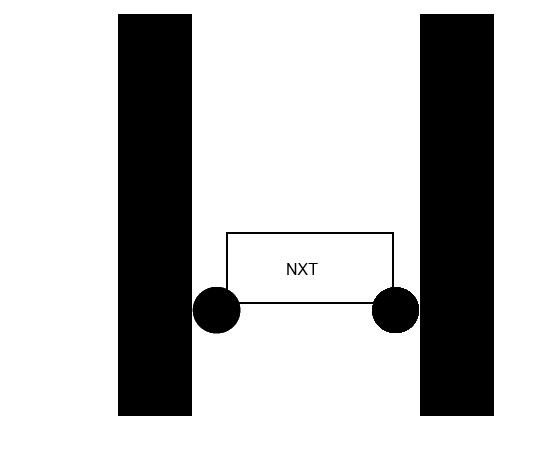
\includegraphics[width=10cm]{images/klettern_skizze}
\end{capfigure}

\section{Aufgabenstellung}
Der Abstand zwischen den Wänden wird beim Workshop bekannt gegeben.

Der Roboter muss ohne zusätzliche Teile die Wand nach oben gelangen.
\section{Lösung}